\documentclass[12pt]{report}
\usepackage{graphicx} % Required for inserting images
\linespread{1.2}

\usepackage[dvipsnames]{xcolor}
\usepackage{tikz}
\usepackage[breakable]{tcolorbox}
\usepackage{colortbl}
\appto{\bibsetup}{\raggedright}

\tikzstyle{mybox} = [draw=BrickRed, fill=BrickRed!5, ultra thick, rectangle, rounded corners, inner sep=10pt, inner ysep=15pt, text width=0.90\textwidth, align=left] 
\tikzstyle{boxtitle} = [fill=BrickRed, text=Apricot!20, ultra thick, rectangle, rounded corners, inner sep=10pt, inner ysep=8pt, text width=0.90\textwidth]

\newcommand{\BoxDef}[2]{%
\vspace*{10px}
\noindent

\begin{center}
\begin{tikzpicture}
    \node[mybox](box){\rule{0pt}{30pt}\ignorespaces#2\unskip};
    \node[boxtitle, anchor=north west] at (box.north west) {\textbf{#1}};
\end{tikzpicture}
\end{center}
}

\newcommand{\colorred}[1]{\textcolor{BrickRed}{#1}}
\newcommand{\colorgreen}[1]{\textcolor{OliveGreen}{#1}}

\newcommand{\ceil}[1]{\left\lceil#1\right\rceil}

\usepackage[hidelinks]{hyperref}
\usepackage{amssymb}
\usepackage{amsmath}
\usepackage{bm}
\usepackage[top=2.5cm, bottom=2.5cm, left=3cm, right=3cm, centering]{geometry}
\usepackage{algorithm}
\usepackage{algpseudocode}
\usepackage{tabularx}
\usepackage{tabularray}

\begin{document}

\begin{titlepage}
\hrule
\vspace{15pt}
\begin{center}
    \Huge{\textbf{\Huge \textbf{Advanced Databases 23-24}} \\ Notes}\\
\end{center}
\vspace{15pt}
\hrule
\vfill
\hrule
\begin{center}
    \Large University of Pisa \\ M.Sc. in Computer Science
\end{center}
\end{titlepage}

\tableofcontents

\chapter{Introduction}

The most common use of information technology is to store and retrieve data, be it text, images, video, or audio files. As the amount of data generated by several processes increases as time goes on, storage systems must evolve to guarantee reliable access to the data, as well as fast and efficient retrieval. Data is typically stored into \textbf{databases} (\textbf{DBs}), which are housed in a permanent memory.

The technology on which permanent memory is based uses magnetic \textbf{disks}, containing a set of platters that rotate at relatively slow speeds (compared to CPU speed), which can be interacted with by using heads attached to moving arms. Each platter has on both surfaces a set of rings, called \textbf{tracks}, which, except for the innermost and outermost ones, are used to store information. Each track is subdivided into \textbf{sectors} of the same size, which correspond to the smallest unit of transfer allowed by the hardware. Typical sector sizes are 512 bytes, 1 KB, 2 KB, or 4 KB. There are from 500 to 1000 sectors per track, and about 100K tracks per surface of a single platter.

The \textbf{access time} needed to read a section of the disk is given by the seek time (needed to move the head), the rotational delay (given by the spinning of the disk itself), and the transfer time (needed to read/write the data). These operations take several milliseconds to be completed, which are definitely slower than any operation relative to the \textbf{main memory} (\textbf{RAM}), taking only a few nanoseconds in total. 

Despite this disparity, disks are still today the preferred technology to store data. Main memory is, in fact, volatile: once the machine stops receiving electricity powering it on, any information on the RAM is lost forever. On the other hand, disks provide reliable storage: the information written on them can be retrieved even if the machine is turned off and on. A newer technology, called \textbf{solid state storage}, and, in particular, \textbf{flash memory}, has risen in popularity in the last years. It provides the reliability of disks and much faster operations, although they still haven't become the new standard since they tend to be expensive.
\chapter{Overview of a DBMS}

This chapter will give a general overview of the structure of a centralized \textbf{DBMS} (\textbf{Data Base Management System}) based on the relational data model, describing its components and their respective functionalities.

\section{Architecture}

A database is a collection of homogeneous sets of data, with relationships defined among them, stored in permanent memory, and used via a DBMS.

\BoxDef{DBMS}{
A DBMS is a software that provides the following functionalities:
\begin{itemize}
    \item A language to describe the \textbf{schema} of the database (a collection of definitions that describe the data structures), restrictions on the allowed data types, and the relationships among data sets;
    \item The data structures for storage and efficient retrieval of large amounts of data;
    \item A language to guarantee secure access to the data only to authorized users;
    \item A \textbf{transactions} mechanism to protect data from HW/SW malfunctions and errors during concurrent access.
\end{itemize}
}

The architecture of a DBMS provides the following basic components:
\begin{itemize}
    \item The \textbf{Storage Engine}, which includes modules supporting:
    \begin{itemize}
        \item \textbf{Permanent Memory Manager};
        \item \textbf{Buffer Manager};
        \item \textbf{Storage Structures Manager};
        \item \textbf{Access Methods Manager};
        \item \textbf{Transaction and Recovery Manager};
        \item \textbf{Concurrency Manager}.
    \end{itemize}

    \item The \textbf{Relational Engine}, which includes modules supporting:
    \begin{itemize}
        \item \textbf{Data Definition Language};
        \item \textbf{Query Manager};
        \item \textbf{Catalog Manager}.
    \end{itemize}
\end{itemize}
In real systems the functionalities of these modules are not completely separated in different components (as in Figure \ref{fig:DBMS_schema}), but this overview can help in understanding the purpose of each of them. 

\begin{figure}[h]
    \centering
    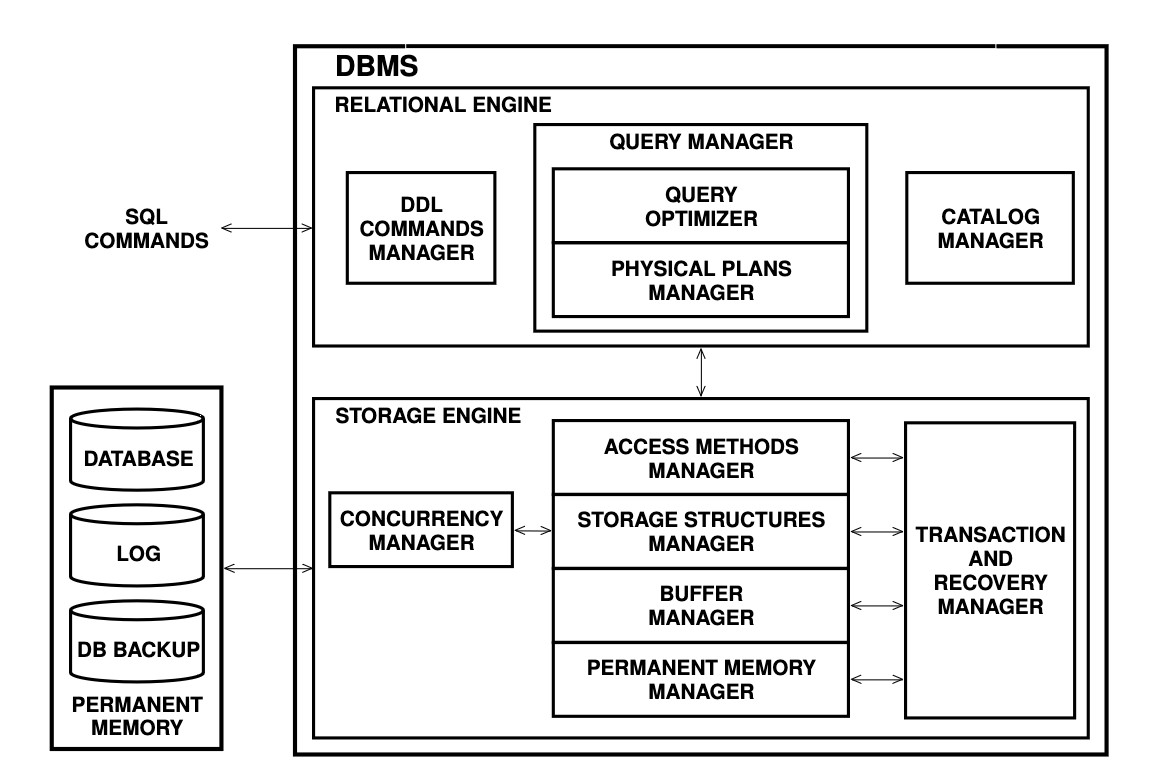
\includegraphics[width=0.75\linewidth]{img/DBMS schema.png}
    \caption{The architecture of a DBMS.}
    \label{fig:DBMS_schema}
\end{figure}

\subsection{Permanent Memory Manager}

The PMM manages page allocation and deallocation on disk storage. It hides the disk characteristics and the operating system, as it provides an abstraction of the memory as a a set of databases, each consisting of a set of logical files of \textbf{physical pages} (or blocks) of fixed size. The physical pages of a file are numbered consecutively starting from 0, and their number can grow dynamically with the only limitation being the available space in the permanent memory.
\chapter{Access Method Management}

The Access Methods Manager provides an interface with several operations to interact with the organizations and indexes implemented by the Storage Structure Manager, so that data can be transferred between main and permanent memory. The language used to implement these operations transform the machine into an \textbf{abstract database machine}, called the database management system. Abstract database machines are divided into two parts:
\begin{itemize}
    \item \textbf{Relational Engine}, or abstract machine for the logical data model. Includes modules to support the execution of SQL commands;
    \item \textbf{Storage Engine}, or abstract machine for physical data model. Includes modules to execute operations on the data in permanent memory.
\end{itemize}

\section{Storage Engine}

The interface of the Storage Engine depends on the data structures used in permanent memory. Normally, it is not directly available to the user, who will instead interact with the Relational Engine which in turn will communicate with the Storage Engine. We will consider an interface inspired by that of the relational system JRS, which stores relations into heap files and provides B$^+$-tree indexes.

\paragraph{Data and Transactions}

\begin{itemize}
    \item $beginTransaction : null \mapsto TransactionId$
    
    \item $commit : TransactionId \mapsto null$
    
    \item $abort : TransactionId \mapsto null$
    
    \item $createDB : Path \times DBName \times TransactionId \mapsto DB$
    
    \item $createHF : DB \times Path \times HFName \times TransactionId \mapsto HF$
    
    \item $createIdx : DB \times Path \times IdxName \times HFName \times Attr \times Ord \times Unique \times TransactionId \mapsto Idx$
    
    \item $dropBD : DBName \times TransactionId \mapsto null$
    
    \item $dropHF : HFName \times TransactionId \mapsto null$
    
    \item $dropIdx : IdxName \times TransactionId \mapsto null$
\end{itemize}

\paragraph{Heap File}

\begin{itemize}
    \item $HFopen : DB \times HFName \times TransactionId \mapsto HF$

    \item $HFCcose: HF \mapsto null$

    \item $HFgetRecord : HF \times RID \mapsto Record$

    \item $HFdeleteRecord : HF \times RID \mapsto null$

    \item $HFupdateRecord : HF \times RID \times FieldNum \times NewField \mapsto null$

    \item $HFinsertRecord : HF \times Record \mapsto RID$

    \item $HFgetNPage : HF \mapsto int$

    \item $HFgetNRec : HF \mapsto int$
\end{itemize}

\paragraph{Indexes}

\begin{itemize}
    \item $Iopen : DB \times IdxName \times TransactionId \mapsto Idx$

    \item $Iclose : Idx \mapsto null$

    \item $IdeleteEntry : Idx \times Entry \mapsto null$ ($Entry = Value \times RID$)

    \item $IinsertEntry : Idx \times Entry \mapsto null$
    
    \item $IgetNKey : Idx \mapsto int$
    
    \item $IgetNLeaf : Idx \mapsto int$

    \item $IgetMin : Idx \mapsto Value$

    \item $IgetMax : Idx \mapsto Value$
\end{itemize}

\section{Access Method Operators}

The following operations transfer data between main and permanent memory. Records of a heap file or of an index are accessed by scans: a heap file scan operator reads each record one after the other, while an index scan operator provides a way to efficiently retrieve the RID of the records. Heap file and index scan operators are implemented using a \textbf{cursor} (or \textbf{iterator}), which is an object with methods that can return one record at a time and move across records. The typical structure of program that scans heap files/indexes is:
\begin{algorithm}
\caption{Typical structure of program that uses scan operators.}
\begin{algorithmic}[1]
    \While{$! C.isDone()$}
        \State $Val = C.getCurrent()$
        \State $\dots$
        \State $C.next()$
    \EndWhile
\end{algorithmic}
\end{algorithm}
Here $C$ is the cursor object.

\paragraph{Heap File Scan}

\begin{itemize}
    \item $HFSopen : HF \mapsto HFS$

    \item $HFSisDone : HFS \mapsto bool$

    \item $HFSgetCurrent : HFS \mapsto RID$

    \item $HFSnext : HFS \mapsto null$

    \item $HFSreset : HFS \mapsto null$

    \item $HFSclose : HFS \mapsto null$
\end{itemize}

\paragraph{Index Scan}

\begin{itemize}
    \item $ISopen : Idx \times fstKey \times lstKey \mapsto IS$

    \item $ISisDone : IS \mapsto bool$

    \item $ISgetCurrent : IS \mapsto null$

    \item $ISreset : IS \mapsto null$

    \item $ISclose : IS \mapsto null$
\end{itemize}
\chapter{Physical Relational Operators}

One of the most important components in a DBMS is the \textbf{Query Manager}, which is responsible of scheduling queries and directing them to the correct tables. Part of the Query Manager is the \textbf{Query Optimizer}, which has the task of determining how to execute a query in the most efficient way possible, considering the physical parameters involved, the data organization, and the presence or absence of indexes.

This chapter will deal with how different physical operators are implemented, for the following operations:
\begin{itemize}
    \item Projection;
    \item Selection;
    \item Grouping;
    \item Set operations;
    \item Join.
\end{itemize}
Then, it will discuss how the optimizer uses these operators to generate efficient physical plans. In general, the problem will be studied under certain assumptions, illustrated in the next sections.

\section{Selectivity Factors}

The selectivity factor of a condition is an estimate of the percentage of the records in a relation which satisfy that condition. The simplest way to estimate this percentage is by assuming the data is uniformly distributed. The selectivity factor of different conditions in reported in table \ref{tab:sf-cond}. The last column is a constant value that is used if not enough information is known to calculate the actual $sf$, or when the attribute is non-numeric. 
\begin{table}[h]
\centering
\SetTblrInner{rowsep=5pt}
    \begin{tblr}{
        hlines,
        vlines,
        columns={145pt, c, m},
        column{1}={80pt}
    }
        Condition & Calculated $sf$ & Approx. $sf$ \\
    \hline
        $A = v$ & $\dfrac{1}{N_{key}}$ & $\dfrac{1}{10}$ \\
        $A > v$ & $\dfrac{\max(A) - v}{\max(A) - \min(A)}$ & $\dfrac{1}{3}$ \\
        $A < v$ & $\dfrac{v - \min(A)}{\max(A) - \min(A)}$ & $\dfrac{1}{3}$ \\
        $v_1 < A < v_2$ & $\dfrac{v_2 - v_1}{\max(A) - \min(A)}$ & $\dfrac{1}{4}$ \\
        $A_1 = A_2$ & $\dfrac{1}{\max(N_{key}(A), N_{key}(B))}$ & $\dfrac{1}{10}$ \\
        $\psi_1 \land \psi_2$ & $sf(\psi_1) \times sf(\psi_2)$ & - \\
        $\psi_1 \lor \psi_2$ & $sf(\psi_1) + sf(\psi_2) -$ $sf(\psi_1) \times sf(\psi_2)$ & - \\
    \end{tblr}
    \caption{Selectivity factors of different conditions.}
    \label{tab:sf-cond}
\end{table}

In many cases, however, attribute values follow non-uniform distributions, making these estimates wrong. The selectivity factor of a condition can be better approximated by knowing the actual distribution of the data, but storing the information needed to have full knowledge about it would occupy too much space. The solution preferred by DBMSs is to use an histogram with binned ranges of values in order to approximate the actual distribution.

There's two types of histograms: \textbf{equi-width} and \textbf{equi-height}. Equi-width histograms are obtained by binning values so that each bin has the same amount of elements $n$. For each bin, the sum of the counts of all elements inside that bin is stored. To find the selectivity factor for an equality search given a value $v$, it will be given by the sum associated with the bin $v$ belongs to, divided by $n$. For inequality/range searches, the selectivity factor will consider the sum associated with all the bins completely included in the range, plus the term that is given by the bin(s) corresponding to the extreme(s) of the condition.

The problem with equi-width histograms is that while they provide better approximations than a blind uniform distribution assumption, they are not able to correctly approximate the distribution of data to a sufficiently high precision. This is why equi-height histograms are used instead. These histograms are divided into bins such that the sum of counts of values within each (their ``height'') is equal across all of them. To store this type of histogram, the only information needed is the number of elements in each bin.

\begin{figure}[h]
    \centering
    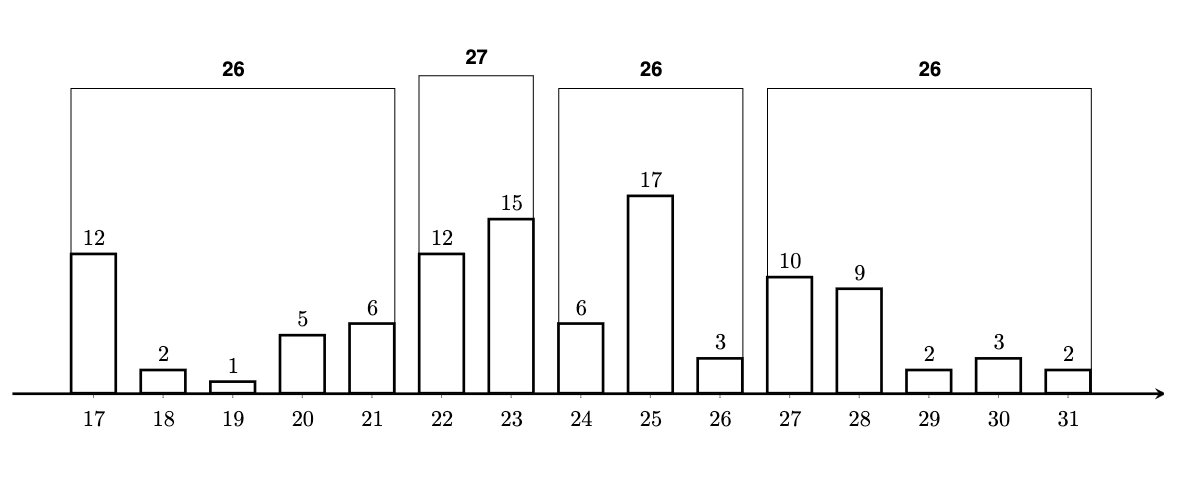
\includegraphics[width=0.7\linewidth]{img/equiheight.png}
    \caption{An equi-height histogram.}
    \label{fig:equi-height}
\end{figure}

Still, the approximation done by these histograms may not be accurate if the distribution within a bin is not uniform. For example, in Image \ref{fig:equi-height}, the third bin has follows a Gaussian distribution. If a query requests all records whose values for that attribute is equal to 24, the selectivity factor approximation will be much higher than the real one; if a query instead requests records with value 25, the approximation will be much lower.

\section{Physical Operators}

\subsection{Operators for Relation}

\paragraph{TableScan($R$)}
Returns all the records in $R$, in the same order as they are stores. It costs
\begin{equation*}
    C = N_{pag}(R)
\end{equation*}
The result size is
\begin{equation*}
    E_{rec} = N_{rec}(R)
\end{equation*}

\paragraph{SortScan($R, \{A_i\}$)}
Returns all the records in $R$ sorted in ascending order on the attribute $A_i$. Sorting is done with a merge sort algorithm. It costs
\begin{equation*}
    C = \begin{cases}
        N_{pag}(R) & N_{pag}(R) < B \\
        3 \times N_{pag}(R) & N_{pag}(R) \leq B \times (B-1) \\
        N_{pag}(R) + 2 \times N_{pag}(R) \times \ceil{log_{B-1}(N_{pag}(R) / B)} & \text{else}
    \end{cases}
\end{equation*}
The result size is
\begin{equation*}
    E_{rec} = N_{rec}(R)
\end{equation*}

\paragraph{IndexScan($R, I$)}
Returns the records of $R$ sorted by the attribute the index $I$ is defined on. It costs
\begin{equation*}
    C = \begin{cases}
        N_{leaf}(I) + N_{pag}(R) & \text{if $I$ is clustered} \\
        N_{leaf}(I) + N_{rec}(R) & \text{if $I$ is on a key of $R$} \\
        N_{leaf}(I) + \ceil{N_{key}(I) \times \phi(\ceil{N_{rec}(R) / N_{key}(I)}, N_{pag}(R))} & \text{else}
    \end{cases}
\end{equation*}
The result size is
\begin{equation*}
    E_{rec} = N_{rec}(R)
\end{equation*}

\paragraph{IndexSequentialScan($R, I$)}
Returns the records of $R$, stored with the primary organization $I$, sorted in ascending order on the primary key values. It costs
\begin{equation}
    C = N_{leaf}(I)
\end{equation}
The result size is
\begin{equation*}
    E_{rec} = N_{rec}(R)
\end{equation*}

\subsection{Operators for Projection}

\paragraph{Project($O, \{A_i\}$)}
Projects the records of $O$ over the attributes $\{A_i\}$. It costs
\begin{equation*}
    C = C(O)
\end{equation*}
The result size is
\begin{equation*}
    E_{rec} = E_{rec}(O)
\end{equation*}

\paragraph{IndexOnlyScan($R, I, \{A_i\}$)}
Returns the sorted records of $R$, projecting them over the attributes $\{A_i\}$ on which the index $I$ is on (or contains them as prefix). It costs
\begin{equation*}
    C = N_{leaf}(I)
\end{equation*}
If a tuple of values for the attributes $\{A_i\}$ is associated with $n$ different RIDs, it is returned $n$ times. The result will not contain duplicates if the attributes are relation keys (they uniquely identify records). The result size is
\begin{equation*}
    E_{rec} = N_{rec}(R)
\end{equation*}

\subsection{Operators for Duplicate Elimination}

\paragraph{Distinct($O$)}
Returns the records of $O$ eliminating all duplicates. This operator requires that the records of $O$ are \textbf{grouped} (if $r_i = r_j$, and $i < l < j$, then $r_i = r_l = r_j$). When a collection of records is sorted, it is also grouped. It costs
\begin{equation*}
    C = C(O)
\end{equation*}
If there's only one attribute in $O$, then the result size is
\begin{equation*}
    E_{rec} = N_{key}(A)
\end{equation*}
If instead it contains multiple attributes, the result size is
\begin{equation*}
    E_{rec} = \min(|O|/2, \prod_i N_{key}(A_i))
\end{equation*}
This is a pessimistic estimate: it assumes that there is a record for each set of values taken from the attributes in $O$, but this is often not the actual result. For example, imagine a database containing data about students enrolled at a university, and the two attributes represent their first name and last name respectively: it is unrealistic to expect that there will be a different student for each first name-last name combination, since the two attributes are loosely correlated.

\paragraph{HashDistinct($O$)}
Returns the records of $O$ without duplicates using and hash technique. This technique has two phases: \textbf{partitioning} and \textbf{duplicate elimination}. Assume the query processor has $B+1$ buffer pages. In the partitioning phase, for each record in $O$ the hash function $h_1$ is applied, distributing records uniformly across the $B$ pages. Once a page $i$ is full, it is written to the $T_i$ partition file. At the end of the phase, all records will be scattered across $B$ files, each of which contains records with the same hash value; this means that duplicates are found in the same partition.

In the duplicate elimination phase, the process becomes an intra-partition problem. Each $T_i$ file is read page-by-page, eliminating duplicates using the hash function $h_2$. A record is deleted when it collides with another record with the same hash value according to $h_2$ and the two records are identical. Assuming each partition occupies at most $B$ pages, at the end of the partition, the $B$ pages are cleared, and the duplicate elimination is applied to the records in the next partition. If the number of pages is greater than $B$, then a hash-based projection technique is applied recursively by dividing the partition into subpartitions. This degrades performances. The operator costs:
\begin{equation*}
    C = C(O) + 2 \times N_{pag}(O)
\end{equation*}
The result size is the same as Distinct, so
\begin{equation*}
    E_{rec} = N_{key}(A)
\end{equation*}
if there's only one attribute in $O$, and
\begin{equation*}
    E_{rec} = \min(|O|/2, \prod_i N_{key}(A_i))
\end{equation*}
if $O$ contains multiple attributes.

\subsection{Operators for Sort}

\paragraph{Sort($O, \{A_i\}$)}
Returns the records of $O$ sorted on the attributes $\{A_i\}$. The sorting algorithm used is merge sort, so its cost is
\begin{equation*}
    C = \begin{cases}
        C(O) & N_{pag}(R) < B \\
        C(O) + 2 \times N_{pag}(O) & N_{pag}(O) \leq B \times (B-1) \\
        C(O) + 2 \times N_{pag}(O) \times \ceil{log_{B-1}(N_{pag}(O) / B)} & \text{else}
    \end{cases}
\end{equation*}
The result size is
\begin{equation*}
    E_{rec} = N_{rec}(O)
\end{equation*}

\subsection{Operators for Selection}

\paragraph{Filter($O,\psi$)}
Returns the records of $O$ that satisfy the condition $\psi$. It costs
\begin{equation*}
    C = C(O)
\end{equation*}
The result size is
\begin{equation*}
    \ceil{sf(\psi) \times N_{rec}(O)}
\end{equation*}

\paragraph{IndexFilter($R,I,\psi$)}
Returns the records of $R$ that satisfy the condition $\psi$ using the index $I$, defined on the attributes involved in $\psi$, sorted according to $I$. The condition is a predicate or a conjunction of predicates that only involve the attributes found in the prefix of the index search key.

IndexFilter always appears as a leaf node in a physical plan. This operator uses the index to find the sorted set of RIDs of all records that satisfy the condition, then it retrieves the records from disk. The cost can be broken down as
\begin{equation*}
    C = C_I + C_D
\end{equation*}
\begin{itemize}
    \item If the index is clustered:
    \begin{align*}
        &C_I = \ceil{sf(\psi) \times N_{leaf}(I)} \\
        &C_D = \ceil{sf(\psi) \times N_{pag}(R)}
    \end{align*}

    \item If the index is unclustered:
    \begin{align*}
        &C_I = \ceil{sf(\psi) \times N_{leaf}(I)} \\
        &C_D = \ceil{sf(\psi) \times N_{key}(I)} \times \ceil{\Phi(\ceil{N_{rec}(R) / N_{key}(I)}, N_{pag}(R))}
    \end{align*}
    If the index is defined on a key of $R$, then
    \begin{equation*}
        C_D = \ceil{sf(\psi) \times N_{rec}(R)}
    \end{equation*}
\end{itemize}
The result size is
\begin{equation*}
    E_{rec} = \ceil{sf(\psi) \times N_{rec}(R)}
\end{equation*}

\paragraph{IndexSequentialFilter($R,I,\psi$)}
Returns the sorted records of $R$, stored with the primary organization $I$, satisfying the condition $\psi$, which involves only the attributes of the index search key. It costs
\begin{equation*}
    C = \ceil{sf(\psi) \times N_{leaf}(I)}
\end{equation*}
The result size is
\begin{equation*}
    E_{rec} = \ceil{sf(\psi) \times N_{rec}(R)}
\end{equation*}

\paragraph{IndexOnlyFilter($R, I, \{A_i\}, \psi$)}
Returns the sorted records of the projection on $R$ returning only the values for $\{A_i\}$ that satisfy $\psi$, using only the index $I$. It costs
\begin{equation*}
    C = \ceil{sf(\psi) \times N_{leaf}(I)}
\end{equation*}
The result size is
\begin{equation*}
    E_{rec} = \ceil{sf(\psi) \times N_{rec}(R)}
\end{equation*}

\subsection{Operators for Grouping}

\paragraph{GroupBy($O, \{A_i\}, \{f_i\}$)}
Returns the records of $O$ sorted on $\{A_i\}$, applying the aggregation functions $\{f_i\}$. The records in $O$ must already be sorted beforehand. It costs
\begin{equation*}
    C = C(O)
\end{equation*}

\paragraph{HashGroupBy($O, \{A_i\}, \{f_i\}$)}
Returns the records of $O$ grouped by $\{A_i\}$, applying the aggregation functions $\{f_i\}$. The records are not sorted on $\{A_i\}$. The grouping is done using two phases, like HashDistinct. In the first phase, called partitioning phase, a partition is created using the hash function $h_1$; in the second phase, called grouping, the records of each partition are grouped using the hash function $h_2$ applied to all grouping attributes. When two records with the same grouping attributes are found, a step to compute the aggregate function is applied. The operator costs
\begin{equation*}
    C = C(O) + 2 \times N_{pag}(O)
\end{equation*}

For both the previous two operators, the result size is calculated as for the duplicate elimination. If there's only one attribute in $O$, then the result size is
\begin{equation*}
    E_{rec} = N_{key}(A)
\end{equation*}
If instead it contains multiple attributes, the result size is
\begin{equation*}
    E_{rec} = \min(|O|/2, \prod_i N_{key}(A_i))
\end{equation*}

\subsection{Operators for Join}

\paragraph{NestedLoop($O_E, O_I, \psi_J$)}
Joins the external operand $O_E$ with the internal operand $O_I$ with the following algorithm:
\begin{algorithm}
\begin{algorithmic}
    \For{$r \in O_E$}
        \For{$s \in O_I$}
            \If{$\psi_J$}
                \State If $\psi_J$, add $<r,s>$ to the result.
            \EndIf
        \EndFor
    \EndFor
\end{algorithmic}
\end{algorithm} \\
It costs
\begin{equation*}
    C = C(O_E) + E_{rec}(O_E) \times C(O_I)
\end{equation*}
The result size is
\begin{equation*}
    E_{rec} = sf(C_j) \times E_{rec}(O_E) \times E_{rec}(O_I)
\end{equation*}

\paragraph{PageNestedLoop($O_E, O_I, \psi_J$)}
Joins the external operand with the internal operand by scanning $O_I$ once per page of $O_E$ (and not once per record, as for NestedLoop). The algorithm used is the following:
\begin{algorithm}
\begin{algorithmic}
    \For{$p_r$ of $O_E$}
        \For{$p_s$ of $O_I$}
            \For{$r \in p_r$}
                \For{$s \in p_s$}
                    \State If $\psi_J$, add $<r,s>$ to the result. 
                \EndFor
            \EndFor
        \EndFor
    \EndFor
\end{algorithmic}
\end{algorithm} \\
The cost of the operator is
\begin{equation*}
    C = C(O_E) + N_{pag}(O_E) \times C(O_I)
\end{equation*}
The algorithm cost is lower when the external operand is the one with fewer pages.
The result size is
\begin{equation*}
    E_{rec} = sf(C_j) \times E_{rec}(O_E) \times E_{rec}(O_I)
\end{equation*}

\paragraph{BlockNestedLoop($O_E, O_I, \psi_J$)}
Joins the external operand $O_E$ with the internal operand $O_I$ by extending PageNestedLoop using more memory for a group of pages of the external operand. Assume the operands are TableScan of tables $R$ and $S$, and that the query processor has $B+2$ pages in the buffer. $B$ pages are used for the external operand, 1 page for an input page of $S$, and 1 page is reserved as the output buffer. For each record $r$ of a page group of $R$, and for each joining record $s$ of a page in $S$, $<r,s>$ is written to the output buffer page.

The cost of the operator is
\begin{equation*}
    C = N_{pag}(R) + \ceil{N_{pag}(R)/B} \times N_{pag}(S)
\end{equation*}
The cost is lower if the external relation has fewer pages than the internal one. If the $B$ pages are enough to contain one of the two relations, then the cost is reduced to
\begin{equation*}
    N_{pag}(R) + N_{pag}(S)
\end{equation*}
The result size is
\begin{equation*}
    E_{rec} = sf(C_j) \times E_{rec}(O_E) \times E_{rec}(O_I)
\end{equation*}
This operator is not convenient to use when the operators require too many pages (i.e., $N_{pag}R \geq B^2$).

\paragraph{IndexNestedLoop($O_E, O_I, \psi_J$)}
This operator requires that there is an index on the join column of the internal operand, and performs a join with the following algorithm:
\begin{algorithm}
\begin{algorithmic}
    \For{$r \in O_E$}
        \For{$s \in$ IndexFilter($O_I, I, O_E.e1 = O_I.i1$)}
            \State Add $<r,s>$ to the result.
        \EndFor
    \EndFor
\end{algorithmic}
\end{algorithm} \\
It costs
\begin{equation*}
    C = C(O_E) + E_{rec}(O_E) \times (C_I + C_D)
\end{equation*}
where $C_I$ and $C_D$ are the costs to retrieve the relevant index records and the data from disk. If the internal operand is an IndexFilter($S,I,\psi_J$), the result size is
\begin{equation*}
    E_{rec} = \ceil{sf(\psi_J) \times E_{rec}(O_E) \times N_{rec}(S)}
\end{equation*}
if instead it is a Filter(IndexFilter($S, I, \psi_J$), $\psi$), the result size is
\begin{equation*}
    E_{rec} = \ceil{sf(\psi_J) \times E_{rec}(O_E) \times (sf(\psi) \times N_{rec}(S))}
\end{equation*}

\paragraph{MergeJoin($O_E, O_I, \psi_J$)}
This operator requires that $O_E$ and $O_I$ are sorted on the same join attributes, and that in the join condition, $O_E.A_i$ is a key of $O_E$. Since this join attribute has distinct values in $O_E$, the algorithm reads the records of $O_E$ one by one, and reads all records of $O_I$ with the same values (which will be found one after the other). This operator costs
\begin{equation*}
    C = C(O_E) + C(O_I)
\end{equation*}
The result size is
\begin{equation*}
    E_{rec} = \ceil{sf(\psi_J) \times E_{rec}(O_E) \times E_{rec}(O_I)}
\end{equation*}

\paragraph{HashJoin($O_E, O_I, \psi_J$)}
Returns the join result with a hash technique in two phases. In the first phase, called partitioning phase, the records of both operands are partitioned using the hash function $h_1$, similarly to HashDistinct. In the second phase, called \textbf{probing} (or \textbf{matching}), for each $B_i$ partition, the records of $O_E$ are read and inserted into the buffer hash table with $B$ pages using the hash function $h_2$. The records of $O_I$ are read one page at a time, $h_2$ is applied to them, and if there is a match with the records in $O_E$, the joined record is added to the result.

Assuming $N_{pag}(O_E)/B < B$ and that the pages are uniform, the cost of the operator is
\begin{equation*}
    C = C(O_E) + C(O_I) + 2 \times (N_{pag}(O_E) + N_{pag}(O_I))
\end{equation*}
where $(C(O_E) + C(O_I) + (N_{pag}(O_E) + N_{pag}(O_I))$ is the cost of the partitioning phase, and $(N_{pag}(O_E) + N_{pag}(O_I))$ is the cost of the probing phase. However, if the pages are not uniform, the resulting partitions will not have the same size, they may not fit in $B$. The cost can be generalized to
\begin{equation*}
    C = (\log_B(N_{pag}(O_E)) \times 2 - 2) \times (N_{pag}(O_E) + N_{pag}(O_I))
\end{equation*}
If $N_{pag}(O_E) < B$, the cost is 0.

The result size is
\begin{equation*}
    E_{rec} = \ceil{sf(\psi_J) \times E_{rec}(O_E) \times E_{rec}(O_I)}
\end{equation*}
\chapter{Query Optimization}

The optimizer is a key component of the Query Manager. Its role is to select the optimal physical plan to execute queries using the operators and data structures provided by the Storage Engine. This chapter will show how functional dependencies are used for not only relational schema design, but also for optimization.

\section{Query Processing and Execution}

In general, there are many strategies to execute a query, in particular when it is complex. The problem of optimizing a query is influenced by the fact that a query can be written in several equivalent ways, and relational algebra operators can be implemented using different physical operators.

Query processing is divided into four stages:
\begin{itemize}
    \item \textbf{Query analysis}, in which the correctness of the SQL query is checked, and the query is translated into its internal form, typically based on relational algebra;

    \item \textbf{Query transformation}, in which the logical plan is transformed into an equivalent one that provides a better query performance;

    \item \textbf{Physical plan generation}, in which alternative physical plans are generated and evaluated, of which the one with the lowest cost is chosen;

    \item \textbf{Query evaluation}, in which the chosen physical plan is executed.
\end{itemize}
Query transformation and Physical plan generation are often considered part of the same phase, and are called Query optimizer.

The most interesting transformations regard Distinct elimination, GroupBy elimination, Where-subquery elimination, and View elimination.

\section{Functional Dependencies}

\BoxDef{Functional Dependency}{
Given a relation schema $R$ and $X,Y$ subsets of attributes of $R$, a functional dependency $X \rightarrow Y$ (read as ``$X$ determines $Y$'') is a constraint such that, for every possible instance $r$ of $R$ and for any two tuples $t_1, t_2 \in r$:
\begin{equation*}
    t_1[X] = t_2[X] \implies t_1[Y] = t_2[Y] 
\end{equation*}
}
A functional dependency is \textbf{trivial} if the consequent contains attributes also found in the antecedent:
\begin{equation*}
    XY \rightarrow X
\end{equation*}
A functional dependency is \textbf{atomic} if the consequent is composed of only one attribute:
\begin{equation*}
    X \rightarrow A
\end{equation*}
A functional dependency $X \rightarrow A$ is \textbf{canonical} if:
\begin{equation*}
    X \rightarrow A
\end{equation*}
holds true, but
\begin{equation*}
    X' \rightarrow A, \ \forall X' \subset X
\end{equation*}
does not. Every non-trivial dependency also contains one or more canonical dependencies, obtained by removing extraneous attributes. \\
A \textbf{key} is a set of attributes $K$ such that:
\begin{equation*}
    K \rightarrow T
\end{equation*}
holds and is canonical. \\
The \textbf{union rule} states that:
\begin{equation*}
    X \rightarrow A_1 \dots A_n \iff X \rightarrow A_1, \dots, X \rightarrow A_n
\end{equation*}
To specify that an attribute has a constant value for all tuples, the rule used is:
\begin{equation*}
    \emptyset \rightarrow Y
\end{equation*}

\BoxDef{Logical Implication}{
Given a set of functional dependencies $F$ on a relation schema $R$, a functional dependency $X \rightarrow Y$ is derived (implied) from $F$ if every instance of $R$ that satisfies $F$ also satisfies $X \rightarrow Y$:
\begin{equation*}
    F  \vdash X \rightarrow Y
\end{equation*}
This property holds if $X \rightarrow Y$ can be derived from $F$ using any of \textbf{Armstrong's axioms}:
\begin{itemize}
    \item $Y \subseteq X \implies X \rightarrow Y$ (Reflexivity)
    \item $X \rightarrow Y, Z \subseteq T \implies XZ \rightarrow YZ$ (Augmentation)
    \item $X \rightarrow Y, Y \rightarrow Z \implies X \rightarrow Z$ (Transitivity)
\end{itemize}
}
To test whether a functional dependency is implied by a set of functional dependencies, the \textbf{closure} of the antecedent can be calculated.
\BoxDef{Closure of Attribute Set}{
Given a schema $R <T,F>$, and $X \subseteq T$, the closure of $X$ is:
\begin{equation*}
    X^+ = \{A_i \in T | F \vdash X \rightarrow A_i\}
\end{equation*}
}
The following theorem holds true.
\BoxDef{Theorem}{
\begin{equation*}
    F \vdash X \rightarrow Y \iff Y \subseteq X^+
\end{equation*}
}

Consider a query on a set of tables $R_1(T_1), \dots, R_n(T_n)$, such that no attribute name appears in two tables. After joining the tables and performing a Select, assuming the Where condition $C$ is in CNF, these dependencies hold on the final result:
\begin{itemize}
    \item $K_{ij} \rightarrow T_i \ \forall K_{ij}$ key of $T_i$;
    \item $\emptyset \rightarrow A \ \forall A=c$ in $C$;
    \item $A_i \rightarrow A_j$ and $A_j \rightarrow A_i$ $\forall A_i = A_j$.
\end{itemize}

\section{Eliminations}

\subsection{Distinct Elimination}

Distinct normally requires a physical plan with duplicate elimination, and data must be grouped, usually via a sort operation (which is expensive). A query with a Distinct clause is translated into a relational algebra expression with the projection and duplicate elimination operators. To decide whether this duplicate elimination operator is unnecessary, a functional dependency theory algorithm is used. Specifically, the following theorem is used:
\BoxDef{Theorem}{
Let $A$ be the set of attributes of the result and $K$ the union of the attributes of the key for every table used in the query. If $A \rightarrow K$, then the duplicate elimination is unnecessary.
}
To find out whether $A \rightarrow K$, the closure of $A$ is computed.

If the query contains a GroupBy clause, then the theorem holds for $G$ (the grouping attributes) instead of $K$.

\subsection{GroupBy Elimination}

GroupBy also usually requires a sort operation. A GroupBy can be eliminated if either each group only has one record, or if there is only one group. The first case can be tested for as seen for Distinct, since it's equivalent to checking if the result contains duplicates. For the second case, we must check that the value of the grouping attributes is the same for each tuple; this is done by verifying that the closure of the empty set ($\{\}^+$) contains all the grouping attributes. 

If aggregation functions are used, Count will be replaced by 1, and Min($A$), Max($A$), Sum($A$), and Avg($A$) will be replaced by $A$.

\subsection{Where-subquery Elimination}

This is one of the most common and important transformations. In general, to execute these queries, the optimizer will generate a physical plan for the subquery, which will be executed for each record processed by the outer query. We will assume all subqueries  have been converted to an equivalent form using Exists, and that no GroupBy appears in the subquery. Given a query in the form
\begin{figure}[H]
    \centering
    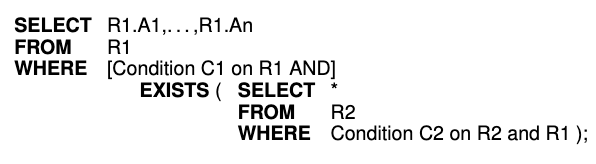
\includegraphics[width=0.75\linewidth]{img/opt_query1.png}   
\end{figure}
\noindent it is equivalent to
\begin{figure}[H]
    \centering
    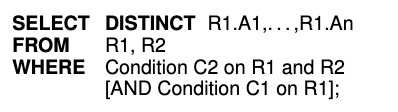
\includegraphics[width=0.5\linewidth]{img/opt_query2.png}
\end{figure}
The Distinct is necessary in the join form when a (1:N) relationship exists between R1 and R2. Note that if only a subset of R1's attributes appears in the Select clause, this transformation will not be correct unless the original query has a Distinct in the outer query.

If the subquery has an aggregation function, then the unnested equivalent requires a GroupBy clause on the projection attributes. A well-known problem is the \textbf{count bug problem}, which arises when the aggregation function is Count. In this case, the unnested query join must be replaced by an outer join.
An outer join is represented by a NATURAL RIGHT JOIN, NATURAL LEFT JOIN, or NATURAL FULL JOIN operator; the first one preserves all records from the left operand, the second one preserves all records from the right operand, and the third one preserves all records.

\begin{figure}[h]
\centering
    \begin{minipage}{0.49\textwidth}
    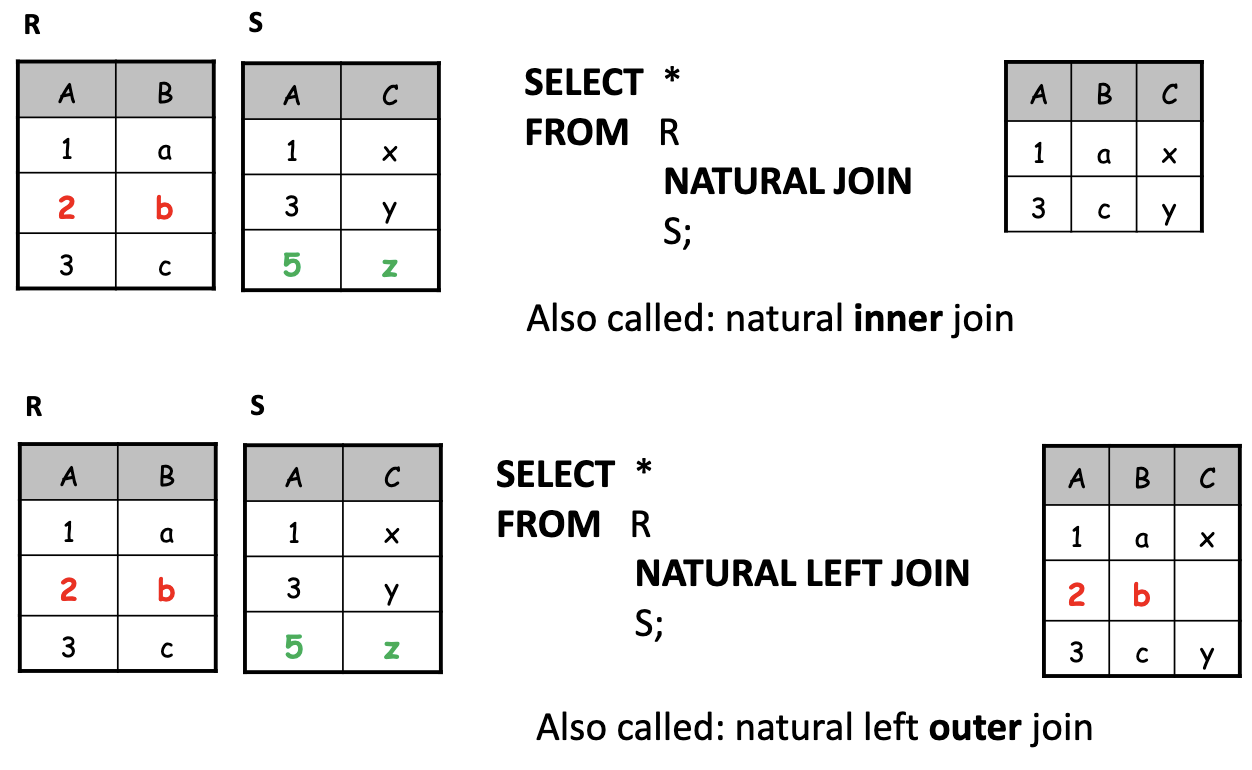
\includegraphics[width=\linewidth]{img/joins1.png}
    \end{minipage} 
    \hfill
    \begin{minipage}{0.49\textwidth}
    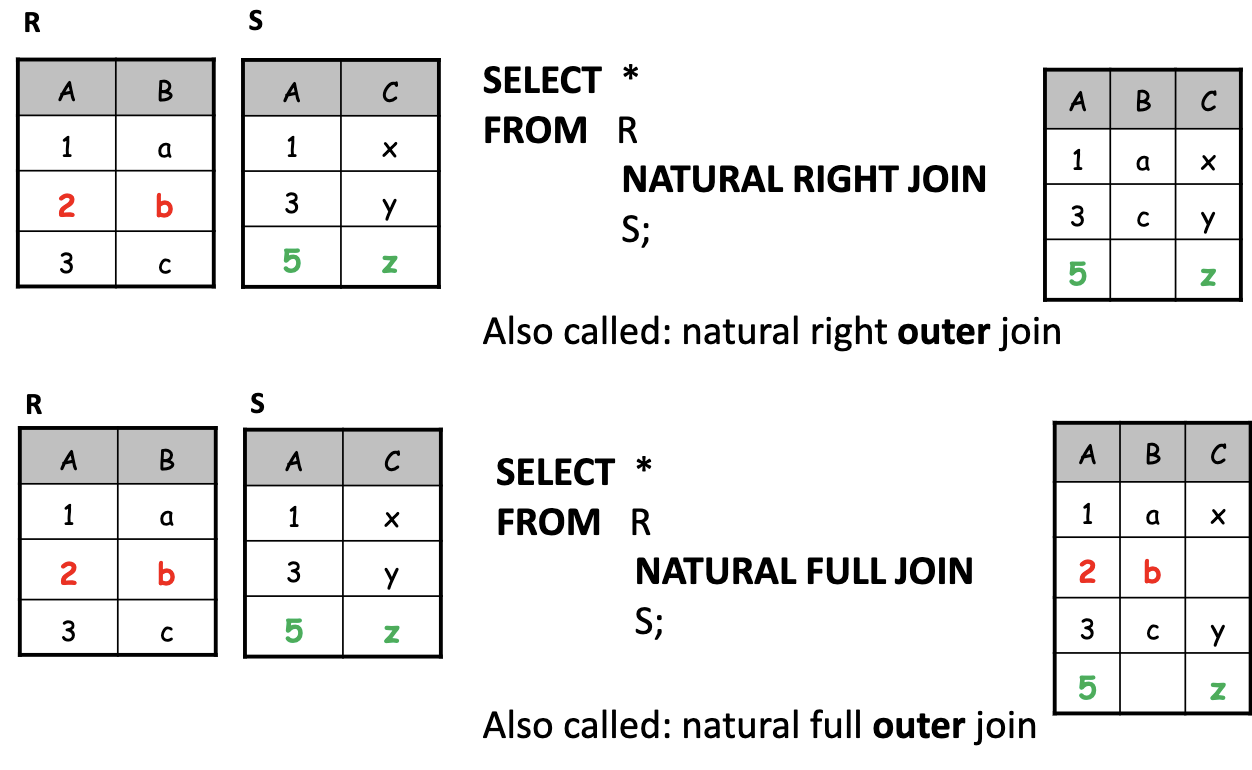
\includegraphics[width=\linewidth]{img/joins2.png}
    \end{minipage}
    \caption{Types of join.}
    \label{fig:joins_in_out}
\end{figure}

\subsection{View Merging}

Complex queries are easier to understand if views are used. The With clause defines temporary views available only to the query in which the clause occurs. When a query generates a view, the optimizer generates a physical sub-plan for the Select that defines the view, and optimizes the query considering the scan as the only operation available for the result of the view; with this technique, the view is optimized separately from the rest of the query.

In the logical plan, the transformation is made by replacing the reference to a view name with the corresponding logical plan. The new logical plan is then rewritten using equivalence rules of relational algebra to put it in the following canonical form:
\begin{equation*}
    \pi^b(\sigma(\gamma(\sigma(^{\bowtie}_J R_i))))
\end{equation*}
The transformation of a query to avoid the use of views defined with a GroupBy generally requires pulling the GroupBy above a join, using the following algebraic equivalence rule:
\begin{equation*}
    ({}_{X_R} \gamma_F(R)) \bowtie_{f_{k} = p_k} S \equiv {}_{X_R \cup A(S)} \gamma_F (R \bowtie_{f_{k} = p_k} S) \,,
\end{equation*}
where $X_R$ is a set of attributes of $R$, $f_k \in X_R$ the foreign key of $R$, and $p_k$ the primary key of $S$ of attributes $A(S)$.

\section{Physical Plan Generation}

With eliminations, a ``random'' physical plan is generated for the query, which is then optimized. Generation, on the other hand, directly finds the best possible physical plan, in two steps: generation of alternative physical query plans, and choice of physical query plan with the lowest estimated cost. To estimate the cost of the entire plan, it is necessary to estimate the cost of the physical operator and the size of the result of every node in the tree (in a bottom-up fashion). The following sections will show how to choose the physical query plan of minimum cost for different types of queries.

\subsection{Single-Relation Queries}

For these queries, the only question to solve is whether to use indexes when accessing the data instead of performing a simple TableScan. Some relations may have single or multiple indexes defined on one or more of their attributes; in that case, the cost of reading the entire table is compared against the cost of reading the index and retrieving the data using the RIDs contained in the index. Usually, using an index is better if the selectivity factor of the query is restrictive enough. A special case happens when the attributes appearing in the Select are included in the prefix of the key of an index of the relation; the query can be evaluated by only reading the index itself, which is much faster than reading the whole table. 

\subsection{Multiple-Relation Queries}

The most important issue in these queries is the order in which the relations are joined. Every permutation of relations yields the same result but corresponds to a different plan; given $n$ relations, there are $n!$ different permutations, each of which generates a huge number of candidates depending on the specific joins performed in the plan. Additionally, there are different choices for the specific physical operator used to implement the join, increasing the total number of possible plans.

The full search in the space of candidates starts by finding which relation is cheaper to access (representing the operator as a standalone plan). Then, the second cheapest plan is chosen among the ones not selected in the previous step and the ones that would be generated by a join of the previously chosen relation with a different one, and so on until the entire query is covered by the physical plan. At each step, the only plans evaluated are the ones behind a so-called ``frontier'', meaning all plans that are direct children of either the (empty) root of the entire search or a plan that has been selected as a minimum cost one.

This algorithm can be incredibly efficient for simpler queries and incredibly slow for complex ones. In the latter case, the algorithm will tend to backtrack to higher levels in the ``tree'' of physical plans explored. A simple pseudocode for this algorithm is presented below.

\begin{algorithm}
\caption{Full search pseudocode.}
\begin{algorithmic}[1]
    \State Initialize $Plans$ to the best plans to access each relation in the query.
    \Loop
        \State Extract the fastest plan $P$ from $Plans$.
        \If{$P$ is complete}
            \State \Return $P$
        \EndIf
        \For{$R$ not in $P$}
            \State Put the best plan between $P \bowtie R$ and $R \bowtie P$ in $Plans$.
        \EndFor
        \State Remove $P$.
    \EndLoop
\end{algorithmic}
\end{algorithm}

Several heuristics have been proposed that can help speed up the algorithm, meaning that the algorithm may not find the optimal physical plan but one that is good enough. The most commonly used heuristics are:
\begin{itemize}
    \item \textbf{Limitation in the number of successors}: each permutation is evaluated by associating the join operators only to the left, creating \textbf{left-deep} trees, where each node from the root up until the second-to-last level has a join as a left child and a relation as a right child (as opposed to \textbf{right-deep} and \textbf{bushy} trees). A left-deep tree has the advantage of allowing the use of an index nested loop join operator. 

    \begin{figure}[h]
        \centering
        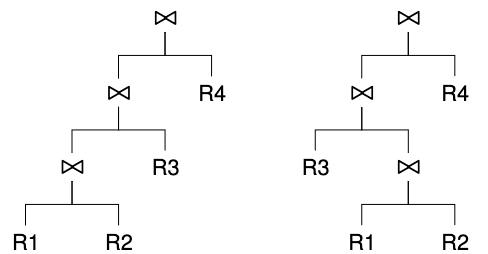
\includegraphics[width=0.5\linewidth]{img/leftdeep_vs_bushy.png}
        \caption{Left-deep tree on the left, bushy tree on the right.}
        \label{fig:ldeep-vs-bushy}
    \end{figure}

    \item \textbf{Greedy search}: once the logical node of minimum cost has been expanded, the other nodes are not considered anymore, avoiding any backtracking. In general, solutions found using a greedy search are suboptimal, but thanks to the fact that it is found in less time, this search is usually the default one used by DBMSs.

    \item \textbf{Iterative full search}: a possibility is to use a mixed approach. The full search is made up to a predetermined number of levels, then the best node to expand is chosen, and, as in the greedy search, the other nodes will not be considered any longer. The full search will continue for the predetermined number of levels, and so on.

    \item \textbf{Interesting orders}: when the merge-join operator is available, and the query result must be sorted because of the presence of an OrderBy or a GroupBy, it is useful to organize the search as follows: at each step, for each logical query subexpression, the preserved query plans will be the one with minimum cost as well as the best plans producing an interesting order of the records potentially useful for the final query plan. 
\end{itemize}

\subsection{Other Queries}

\subsubsection{Queries With GroupBy}

If the GroupBy is necessary, the optimizer produces a physical plan for the Select only, sorting the data on the grouping attributes; this plan is then extended with the physical operator for the GroupBy and the one for the Project over the Select attributes. If an Having clause was specified, the physical plan is also extended with a selection operator, and the GroupBy computes whatever aggregation function used in the Having and Select clauses.

\paragraph{Exchanging with a Join}
If the query requires a Join, it may be convenient to GroupBy before the Join (with the constraint that the GroupBy is done on the same attributes used in the Join); often, however, Joins are submultiplicative, so moving it above the GroupBy may make the plan more expensive. The equivalence rules for this transformation are done under these assumptions:
\begin{itemize}
    \item The tables do not have null values, and primary and foreign keys have only one attribute;

    \item The queries are a single Select with GroupBy and Having, but without any subselect, Distinct, or OrderBy clauses;

    \item The Select includes all grouping attributes.
\end{itemize}
Then, the pre-grouping problem is: when does this equivalence rule:
\begin{equation*}
    {}_X \gamma_F (R \bowtie_{f_k = p_k} S) \equiv (({}_{X'} \gamma_{F'}(R)) \bowtie_{f_k = p_k} S)
\end{equation*}
hold?

The fundamental condition is that the join is unary w.r.t. the attributes $X$, meaning that it produces exactly one record for each value of that attribute. This is true under the following conditions:
\begin{itemize}
    \item Let $C_j$ be the Join condition; then $C_j \vdash X \rightarrow A(S)$, producing one record from $S$ for every group;

    \item Each aggregate function only uses attributes from $R$.
\end{itemize}

\paragraph{Exchanging with a Filter}
For this transformation, we need to find if the following equivalence rule holds:
\begin{equation*}
    \sigma_{\phi}({}_X \gamma_F (E)) \equiv {}_X \gamma_F (\sigma_{\phi}(E))
\end{equation*}
This equivalence rule is typically used when the query contains an Having clause, or it uses a view that specifies a condition on its attributes. There's two possible cases; either the selection is done on the dimensions of a table, or it is done on the results of aggregate functions in the GroupBy. \\
The first case is simple:
\begin{equation*}
    \sigma_{\phi_X} ({}_X \gamma_F (E)) \equiv {}_X \gamma_F (\sigma_{\phi_X} (E))
\end{equation*}
If the restriction is done on the same attributes on which the GroupBy is performed, it can be moved below. However, this rule is rarely used, since these conditions are normally specified in the Where clause and not the Having clause, so they already appear below GroupBys. \\
The second case is more complicated:
\begin{equation*}
    \sigma_{\phi_F} ({}_X \gamma_{AGG(A_1) \ AS \ F_1, \dots, AGG(A_n) \ AS \ F_n} (E))
\end{equation*}
Equivalence rules can be built only in these two case
\begin{gather*}
    \sigma_{\phi_{Mb \geq v}} ({}_X \gamma_{MAX(b) \ AS \ Mb} (E)) \equiv {}_X \gamma_{MAX(b) \ AS \ Mb} (\sigma_{b} \geq v(E))\\
    \sigma_{\phi_{mb \leq v}} ({}_X \gamma_{MIN(b) \ AS \ mb} (E)) \equiv {}_X \gamma_{MIN(b) \ AS \ mb} (\sigma_{b} \leq v(E))
\end{gather*}
\chapter{Transactions}

The Storage Engine offers features aimed at solving recovery and concurrency problems, guaranteeing that each operation performed by the user is executed such that the user does not notice any underlying failure, and that there are no interferences with other operations running concurrently. The solutions to these problems are based on a mechanism called \textbf{transaction}.
\BoxDef{Transaction}{
    A transaction is a sequence of operations on the database and on temporary data, with the following properties:
    \begin{itemize}
        \item Atomicity: only successful transactions change the state of the database; if a transaction is interrupted the database must remain unchanged as if the transaction was never started;

        \item Isolation: when a transaction is executed concurrently with others, the final effect must be the same as if it was executed alone;

        \item Durability: the effects of committed transactions must survive system and media failures.
    \end{itemize}
}
Often, the acronym \textbf{ACID} (\textbf{Atomicity}, \textbf{Consistency}, \textbf{Isolation}, and \textbf{Durability}) is used to refer to the properties of transactions. The Recovery Manager ensures Atomicity and Durability, while the Concurrency Control Manager ensures Isolation. Consistency is guaranteed by the implementation of integrity constraints and code correctness.

For the DBMS, a transaction $T$ requires a number of read/write operations on the database. Each transaction starts and ends with the following transaction operations:
\begin{itemize}
    \item \textit{beginTransaction}, signaling the start of the transaction;
    \item \textit{commit}, signaling the successful termination of the transaction, and requiring the system to make its updates durable;
    \item \textit{abort}, signaling the abnormal termination of the transaction, requiring the system to undo its updates.
\end{itemize}
While a \textit{commit} is only used as a command in the code, \textbf{abort} can be either specified in the code or it can be used by the system. The execution of a \textbf{commit} does not automatically mean that the transaction will successfully terminate, because its updates may not be written on permanent memory. Figure \ref{fig:transaction-states} shows the state transition diagram for transaction execution.
\begin{figure}[h]
    \centering
    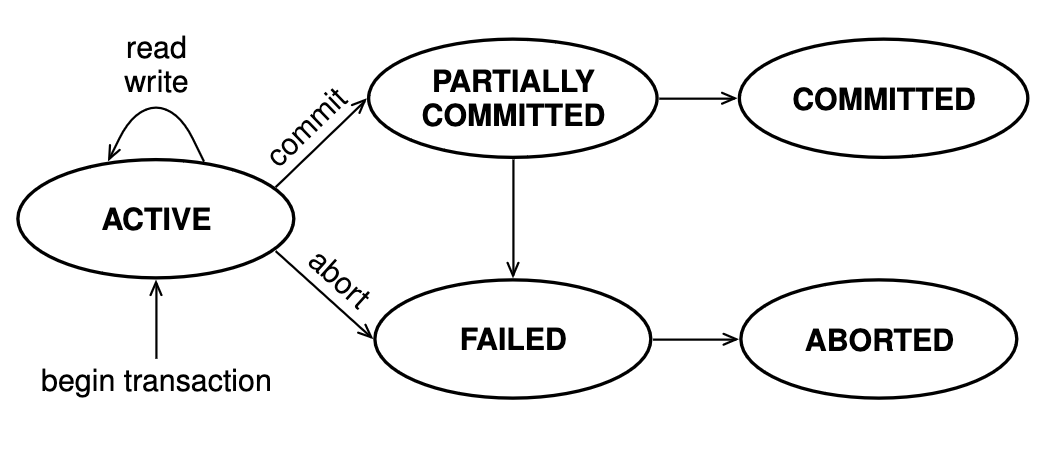
\includegraphics[width=0.5\linewidth]{img/transaction_states.png}
    \caption{State transition diagram for transaction execution.}
    \label{fig:transaction-states}
\end{figure}
To read a page ($r_i[x]$), it is brought into the buffer from the disk (if it's not already in the buffer), and then read. To write a page ($w_i[x]$), an in-memory copy is modified, which will later be written to disk when the Buffer Manager find it appropriate to do so. This delayed writing has to be compatible with Atomicity and Durability, since multiple transactions may want to write to the same page.

\section{Failures}

A database can become inconsistent because of three types of failures:
\begin{itemize}
    \item \textbf{Transaction failure}, an interruption of a transaction which does not damage the content of either the main memory or the permanent memory. A transaction can be interrupted because either it meets certain conditions, it violates integrity constraints, or the concurrency manager chooses to abort it because it is involved in a deadlock;
    
    \item \textbf{System failure}, an interruption (crash) of the system (DBMS or OS) in which the content of the main memory is lost, but the content of the content of the permanent memory remains intact. After crashes occur, the system is restarted, automatically or by an operator;
    
    \item \textbf{Media failure} (also called \textbf{disaster}), an interruption of the system in which content of the permanent memory is lost or damaged. When a media failure happens, the Recovery Manager uses a backup to restore the database.
\end{itemize}
Other than database backups, another protection from failures is represented by \textbf{log files}: these files contain lines recording each transaction operation executed in the system, including aborted transactions. For each transaction, the information written is when it starts, when it commits, when it aborts, and when it modifies a records, specifying the page the record is in, and the old and new values (called \textbf{before image} and \textbf{after image}). Each record is uniquely identified by a LSN (Log Sequence Number), assigned in a strictly increasing order.

A recovery algorithm requires an \textbf{undo} if an update of some committed transaction is stored in the database. An \textit{undo} is needed when a transaction or system failure occurs, copying the before image of the page from the log to the database. A recovery algorithm requires a \textbf{redo} is a transaction is committed before all of its updates are stored in the database (after a system failure), copying the after image in the log to the database.

The downtime of the system is given by the product between the failure rate and the recovery rate. The failure rate cannot be reduced, as we cannot know in advance if a transaction contains an error, or a system/media failure happens. The way to reduce downtime is to reduce recovery time. In practice, this is done via \textbf{checkpoints}. There's different types of checkpoints:
\begin{itemize}
    \item \textbf{Commit-consistent checkpoint}: when a checkpoint starts, the activation of new transactions is suspended, and the system waits the termination of active transactions; all ``dirty'' pages in the buffer are written to permanent memory; the checkpoint is written to the log file, and a pointer to the corresponding record is stored in a special file called \textbf{restart file}. The system then resumes normal activity. This strategy is simple but inefficient, since the system has to regularly stop.

    \item \textbf{Buffer-consistent checkpoint - Version 1}: similar to the previous type, but once the checkpoint starts, it also suspends the execution of currently active transactions. This strategy is more efficient than the previous, but it is still slow because of the buffer flushing operations.

    \item \textbf{No stop checkpoint}: once the checkpoint starts, the checkpoint is written to the log file, along with the ids of currently active transactions; a new thread is started, which scans the buffer and flushes the dirty pages it finds in parallel with the standard transactions, guaranteeing that all pages that were dirty at the beginning of the checkpoint are flushed before its end.
\end{itemize}

\subsection{Recovery from System and Media Failures}

In order to recover the database, the \textit{restart} operator is invoked, bringing the database in its committed state with respects to the execution up to the system failure, and restarting the normal system operations. The first task is done using a recovery algorithm of which a simple version will be described. This algorithm has two phases, \textbf{rollback} and \textbf{rollforward}. In the rollback phase the log is read backwards, to undo updates of transactions that were not terminated before the crash, and to find the identifiers of the transactions which terminated successfully. In particular, two sets are constructed: the \textbf{redo-list} and the \textbf{undo-list}. Until the first checkpoint record is found, these operations are done:
\begin{enumerate}
    \item If a record is (\textit{commit}, $T_i$), $T_i$ is added to the redo-list.
    
    \item If a record is an update of a transaction $T_i$ not in the redo-list, it is added to the undo-list.

    \item If a record is (\textit{begin}, $T_i$), $T_i$ is removed from the undo-list.

    \item If a record is a checkpoint (\textit{CKP}, $L$), for each $T_i \in L$ if $T_i$ is not in the redo-list it is added to the undo-list. If the undo-list in not empty, the rollback phase continues until it is completely emptied.
\end{enumerate}
In the rollforward phase, the log is read onward from the first record after the checkpoint, redoing all operations of the transactions in the redo-list.

The restart is executed at the buffer level, not on the persistent store: undos and redos are done by first loading the data in the buffer, and then pages are eventually flushed in a second time.

The algorithm described above is the standard Undo-Redo algorithm, but there exist variants:
\begin{itemize}
    \item \textbf{NoUndo-Redo}: requires that all the updates of a transaction must be in the database after the transaction has committed. It uses a \textbf{NoSteal (Pin) Policy}, where all the buffers used by transactions are pinned, and those pages will not be flushed to disk until the transaction commit. This way, no operation ever needs to be undone. It is dangerous because it pins all those pages used by the active transactions, limiting the freedom of the buffer manager.

    \item \textbf{Undo-NoRedo}: requires that all the updates of a transaction must be in the database before the transaction has committed. It uses a \textbf{Force} policy, where buffer pages used by transactions are forcibly flushed before committing. This approach has two problems: it does not work for media failures, and it is costly since it requires a lot of writes to disk.

    \item \textbf{NoUndo-NoRedo}: requires that all the updates of a transaction must be in the database neither before nor after the transaction has committed. It uses NoSteal and Force policies.
\end{itemize}
Undo-Redo uses Steal and NoForce policies.

NoUndo-NoRedo requires a way to write many pages atomically. This is done using \textbf{shadow pages}. When a transaction updates a page for the first time, a new database page is created, called \textbf{current page}, with a certain address $p$. The old page in the database is unchanged, and becomes a shadow page. The \textbf{New Page Table} (a copy of the Page Table containing all physical addresses of pages) is updated so that the first element contains the physical address $p$ of the current page. All subsequent write and read operations on that page will operate on the current page.

Once the transaction reaches the commit point, the system substitutes all shadow pages with an atomic actions: first, all the pages updated in the buffer are written to the permanent memory, while the Page Table is left unchanged; then, the descriptor of the database is updated with an atomic operation, replacing the pointer to the Page Table with that to the New Page Table, which becomes the Page Table.

There are some optimizations of the algorithm:
\begin{itemize}
    \item Setting the log granularity at a record level instead of page level;

    \item Buffering the log;

    \item Writing in pages the LSN of the last operation executed;

    \item Logging undo actions;

    \item Adding to each log entry the LSN of the previous entry for the same transaction.
\end{itemize}
\chapter{Concurrency}

When transactions are executed concurrently, their operations are often interleaved, meaning that the execution of the operations of one transaction alternates with the execution of the operations of the other. This may cause interferences that leave the system in an inconsistent state, and it is responsibility of the Concurrency Manager to prevent this from happening. We assume all transactions are consistent, so if a transaction were to be executed in isolation it would not violate any constraint. There are three types of possible conflicts arising during concurrent execution:
\begin{itemize}
    \item \textbf{Dirty Reads (Write-Read conflicts)}: one uncommitted transaction writes on some data $x$, and the other reads that same $x$ after the write operation has been completed. If the first transaction aborts, the changes to $x$ should not have had an effect on the execution of the second one.

    \item \textbf{Unrepeatable Read (Read-Write conflict)}: a transaction reads the same data $x$ twice, but between the two reads, a write operation on $x$ by another transaction is scheduled. The first transaction will read two different values of $x$, despite expecting them to be the same for both reads.

    \item \textbf{Lost Update (Write-Write Conflict)}: two transactions read the value of the same data $x$ (with no conflict), but then both update $x$ with a new value. Whichever transaction gets to update $x$ last is the one whose change will have an effect on the database, regardless of when it started w.r.t. the other one. 
\end{itemize}
A simple way to avoid interference is to allow only \textbf{serializable execution}.
\BoxDef{Serial Execution}{
An execution of a set of transactions $T = \{T_1, \dots, T_n\}$ is serial if, for every pair of transactions $T_i$ and $T_j$, all the operations of $T_i$ are executed before the ones of $T_j$, or vice-versa. 
}
However, serial execution in unpractical, since one transaction is executed at a time, stopping the others from accessing the data for potentially long periods of time. To make sure that the database stays in a consistent state, it is sufficient that the system guarantees that the execution of interleaved transactions is \textbf{serializable}.
\BoxDef{Serializable Execution}{
An execution of a set of transactions $T$ is serializable if it has the same effect in the database of some serial execution of the set of committed transactions $T' \subseteq T$.
}
Aborted transactions are ignored since they should not change the state of the database. Since serial executions are correct, any serializable execution is also correct by virtue of having the same final effect.

\section{Histories}

A transaction is a sequence of read/write operations. An \textbf{history} is used to represent the interleaved execution of multiple transactions.
\BoxDef{History}{
Let $T = \{T_1,\dots,T_n\}$ a set of transactions. A history $H$ on $T$ is an ordered set of operations such that:
\begin{itemize}
    \item The operations of $H$ are those of $T_1,\dots,T_n$;
    \item $H$ preserves the ordering between the operations belonging to the same transaction.
\end{itemize}
}
A history is an actual (or potential) execution order of the operations of a set of transactions; for example, given the transactions:
\begin{align*}
    &T_1 = r_1[x], r_1[y], w_1[x], c_1 \\
    &T_2 = r_2[y], r_2[z], c_2 \\
    &T_3 = w_3[x], w_3[y], c_3 \\
\end{align*}
a history may be:
\begin{equation*}
    H = r_1[x], r_2[y], r_1[y], w_3[x], w_3[y], w_1[x], c_1, r_2[z], c_3, c_2
\end{equation*}
In an history, two operations of different transactions can be \textbf{in conflict}, i.e., they are on the same data item and at least one of them is a write operation. In the example above, $r_1[x]$ and $w_3[x]$ are in conflict.

\BoxDef{Equivalent Histories}{
Two histories $H$ and $L$ are equivalent if:
\begin{itemize}
    \item They are defined on the same set of transactions;
    \item They produce the same final effect on the database.
\end{itemize}
}
A history is serializable if it is equivalent to a serial history. Equivalence between histories can be defined taking only into account the order of operations in conflict:
\BoxDef{c-Equivalent Histories}{
Two histories $H$ and $L$ are c-equivalent (conflict-equivalent) if:
\begin{itemize}
    \item They are defined on the same set of transactions;
    \item They have the same order of operations in conflict of committed transactions.
\end{itemize}
}
This definition of c-equivalence is motivated by the fact that the result of concurrent execution of $T_1,\dots,T_n$ depends only on the order of execution of the operation in conflict: if two operations are not in conflict, they will always have the same final result on the database regardless of their ordering.

\BoxDef{c-Serializable History}{
A history of transactions $T$ is c-serializable if it is c-equivalent to a serial history on the same transactions of $T$.
}
c-serializability always implies serializability, but not vice-versa.

Although it is possible to examine a history $H$ and decide whether or not it is c-serializable using reordering of operations, there is another simpler way to proceed based on the analysis of a particular graph derived from $H$, called \textbf{serialization graph}.
\BoxDef{Serialization Graph}{
Let $H$ be a history of committed transactions $T = \{T_1, \dots, T_n\}$. The serialization graph of $H$, denoted $SG(H)$, is a directed graph such that:
\begin{itemize}
    \item There is a node for every committed transaction in $H$;
    \item There is a directed arc $T_i \rightarrow T_j, i \neq j$, if and only if some operation $p_i$ in $T_i$ appears before and conflicts with some operation $p_j$ in $T_j$.
\end{itemize}
}
Two transactions $T_i$ and $T_j$ in $H$ are in conflict if the arc $T_i \rightarrow T_j$ appears in $SG(H)$.
\BoxDef{c-Serializability Theorem}{
A history $H$ is c-serializable if and only if its serialization graph is acyclic.
}
If the serialization graph is acyclic, a serial schedule can be obtained with a topological ordering on the graph.

\section{Serializability with Locking}

Analyzing the serialization graph can verify a posteriori if a history is c-serializable; in practice, serialization graphs are not constructed. The c-serializability theorem, however, can be used to prove that the scheduling algorithm for the concurrency control used by a scheduler is correct.

\subsection{Strict Two-Phase Locking (2PL)}

Strict Two-Phase Locking is the most commonly used scheduling protocol in commercial systems. Under this protocol, each data item used by a transaction has a lock associated with it, a \textbf{read lock} (shared), or a \textbf{write lock} (exclusive). Two rules are followed:
\begin{itemize}
    \item If a transaction wants to read (write) a data item, it first requests a shared (exclusive) lock on the data item. Before a transaction can access a data item, the scheduler first examines the lock associated with the data item. If no other transaction holds the lock, then the data item is locked; otherwise, the transaction must wait until the lock is released.
    
    \item All locks held by a transaction are released together the moment it commits or aborts.
\end{itemize}
Lock-granting policies are described by the \textbf{compatibility matrix}, where each row corresponds to a lock that is already held on an element $x$ by another transaction, and each column corresponds to the mode of a lock on $x$ that is requested (here ``S'' stands for ``shared'' and ``X'' stands for ``exclusive''):
\begin{table}[h]
    \centering
    \begin{tabular}{|c||c|c|}
    \hline
         & S & X \\
    \hline
    \hline
        S & \colorgreen{y} & \colorred{n} \\
    \hline
        X & \colorred{n} & \colorred{n} \\
    \hline
    \end{tabular}
    \caption{Compatibility matrix for shared/exclusive locks.}
    \label{tab:my_label}
\end{table}
In short, if an item has a read lock, it can receive more read locks but no write locks. If it has a write lock, no more locks of any kind can be placed.

Locks are handled by a scheduler, which tracks all locks granted to transactions and on which data items: each lock is a triple $(T, mode, x)$. When a transaction asks for a lock on an item, it is granted if possible (according to the above table), otherwise the transaction is suspended and added to a \textbf{wait queue} (hashed on the item). Once a transaction commits or aborts, all the locks it held are released, and any waiting transaction is notified according to a specific policy.

\BoxDef{Theorem}{
A strict 2PL protocol ensures c-serializability.
}

\subsection{Deadlocks}

The scheduler needs a strategy to detect \textbf{deadlocks}, situations in which a transaction $T_i$ has locked an item $A$ and requests a lock on item $B$, while at the same time, a transaction $T_j$ has locked item $B$ and requests a lock on item $A$. A deadlock occurs because none of the transactions can proceed.

\subsubsection{Deadlock Detection}

A simple strategy is using a \textbf{wait-for graph} in which each node is a transaction, and a directed edge between two transactions $T_i$ and $T_j$ means that $T_i$ is waiting for $T_j$ to release a lock on one of its objects. If a cycle occurs in the graph, a deadlock has occurred, and one of the transactions involved must abort, usually the youngest (chosen on the basis of some metric, such as newest timestamp, lowest number of locks, etc.).

In real applications, managing this graph can become very expensive. Either the existence of wait cycles may be controlled at predetermined time intervals, or the graph is not constructed and instead a timeout strategy is used: if a transaction waits to get a lock on a data item for more than \textit{timeout}, the scheduler assumes a deadlock has happened and aborts the transaction. This solution, however, causes thrashing: the system may accidentally start killing transactions which are not involved in deadlocks, in turn slowing down transaction execution. In some DBMSs (such as PostgreSQL), a shorter deadlock timeout is used instead; if this timeout expires, the system builds a local wait-for graph for that transaction, and if the graph contains a loop the transaction is killed.

\subsubsection{Deadlock Prevention}

Another strategy that instead prevents deadlocks from ever happening is the following: each transaction $T_i$ receives a timestamp $t_s(T_i)$ when it starts; if $t_s(T_i) < t_s(T_j)$, then $T_i$ is older than $T_j$. Each transaction has a priority assigned to it, such that the older is a transaction, the higher priority it has.

When a transaction $T_i$ requests a lock on a data item that is already locked on by another transaction $T_j$, two algorithms are possible:
\begin{itemize}
    \item \textbf{Wait-Die}: if $T_i$ is older than $T_j$ it waits until $T_j$ terminates, otherwise aborts.

    \item \textbf{Wound-Wait}: if $T_i$ is older than $T_j$ it aborts it, otherwise it waits until $T_j$ terminates.
\end{itemize}
In both cases, when the killed transaction is restarted, it keeps the same priority (timestamp) it had originally. Both algorithms ensure no starvation. Wait-Die tends to roll back more transactions, but those transactions are also the ones who tend to have done less work since they're younger.

Wait-Die and Wound-Wait are easier to implement than wait-for graphs, and they also tend to kill a huge amount of transaction (as opposed to wait-for graphs who only kill transactions which are presumed to be involved in a deadlock).

\section{Serializability without Locking}

The previous methods are called \textbf{pessimistic}, because they assume that operations of different transactions are very likely to conflict, and act accordingly. Methods that don't use locks are called \textbf{optimistic}: transactions are free to execute their operations, and the system only controls that no errors have happened.

One such method, used by Oracle, is \textbf{snapshot isolation}. In this solution, all reads and writes are done without locks. Each transaction $T_i$ reads the data out of a database version called \textbf{snapshot}, containing the state of all data items as they were modified by all transactions committed before it. All the write operations done by the transaction are collected in a dedicated \textbf{write set} $WS_i$ and they are visible only by $T_i$ but not other transactions. If a transaction executes a write, it can only commit if its write set does not intersect with another committed transaction's write set. If the intersection is not empty, the transaction is aborted: this is called the ``First-Committer-Wins'' rule.

This solution permits non-serializable executions.

\section{Multiple-Granularity Locking}

The locking techniques presented up until now assume that locks are taken for single records. In real applications, transactions may operate on collections of records, so these record-level locks are not enough to guarantee a consistent state of the database. On the other hand, if only table-level locks are provided by the DBMS, transactions that only write on single records will have to lock the entire table they are found in, slowing down execution.

Other techniques have been developed to support locks with different granularity (database, files, page, record, fields), such that an inclusion relationship is defined across the levels. If a transaction gets an \textbf{explicit} lock on a data object, it also has an \textbf{implicit} lock on any ``child'' object as well; i.e., if a transaction has a lock on a table, it also has a lock on its records and each record's field. Low granularity locks allow more concurrency, but also cause more lock overhead and higher deadlock probability. High granularity locks allow less concurrency, but cause less overhead and less chance of deadlock.

To manage these locks, the $S$ and $X$ locks are not enough, so a new type is introduced, called \textbf{intention locks}. If a data object is locked in an intention mode, explicit locking is done at a finer granularity. Before a transaction can acquire an explicit lock on the object, it must also already hold an intention lock on all ancestors of that object in the granularity hierarchy. The intention lock types are:
\begin{itemize}
    \item \textbf{Intentional Shared lock} (\textbf{IS}): allows the explicit locking of the object's descendants in $S$ or $IS$ mode;

    \item \textbf{Intentional Exclusive lock} (\textbf{IX}): allows the explicit locking of the object's descendants in $S$, $IS$, $X$, $IX$, or $SIX$ mode;

    \item \textbf{Shared Intentional Exclusive lock} (\textbf{SIX}): implicitly locks all descendants of the object in $S$ mode, and allows the explicit locking of the object's descendants in $X$, $SIX$, or $IX$ mode.
\end{itemize}
The need for the $SIX$ lock is justified by the fact that some transactions may want to only read an object higher in the hierarchy, but write on objects lower in the hierarchy. If only $S$ and $IX$ locks were used, the transaction would have to hold both those lock types on the object higher in the hierarchy. The compatibility table for these locks is the one below (where the rows represent locks already held, and columns are locks requested by some other transaction).

\begin{table}[h]
    \centering
    \begin{tabular}{|c||c|c|c|c|c|}
    \hline
         & S & X & IS & IX & SIX \\
    \hline
    \hline
        S & \colorgreen{y} & \colorred{n} & \colorgreen{y} & \colorred{n} & \colorred{n} \\
    \hline
        X & \colorred{n} & \colorred{n} & \colorred{n} & \colorred{n} & \colorred{n} \\
    \hline
        IS & \colorgreen{y} & \colorred{n} & \colorgreen{y} & \colorgreen{y} & \colorgreen{y} \\
    \hline
        IX & \colorred{n} & \colorred{n} & \colorgreen{y} & \colorgreen{y} & \colorred{n} \\
    \hline
        SIX & \colorred{n} & \colorred{n} & \colorgreen{y} & \colorred{n} & \colorred{n} \\
    \hline
    \end{tabular}
    \caption{Compatibility matrix of multi-granularity locks.}
    \label{tab:multi-granularity-locks}
\end{table}

A problem that arises with multi-granularity locks is \textbf{phantom locking}. Imagine two transactions, $T_1$ and $T_2$, which are executing the following operations:
\begin{itemize}
    \item $T_1$: SELECT * FROM Students
    \item $T_2$: insert into Students values (100, 'Rossi')
    \item $T_2$: commit
    \item $T_1$: SELECT * FROM Students
\end{itemize}
$T_1$ locks the table record by record. Even if strict 2PL protocol is used, this history is still possible. This is because even if $T_1$ has a lock on the data objects in the table Students, $T_2$ is not updating or deleting an existing record, but inserting a new one, and $T_1$ obviously cannot lock an object that cannot exist yet.

The same problem can be seen for the following cases:
\begin{itemize}
    \item $T_1$: SELECT * FROM Students WHERE Surname='Rossi'
    \item $T_2$: insert into Students values (100, 'Rossi')
    \item $T_2$: commit
    \item $T_1$: SELECT * FROM Students WHERE Surname = 'Rossi'
\end{itemize}
and
\begin{itemize}
    \item $T_2$: DELETE FROM Students WHERE Surname='Rossi'
    \item $T_1$: SELECT * FROM Students WHERE Surname='Rossi'
    \item $T_2$: abort
    \item $T_1$: SELECT * FROM Students WHERE Surname = 'Rossi'
\end{itemize}
In the latter case, the records on which an exclusive lock is held by $T_2$ are deleted, thus deleting the lock as well.

To fix this problem, a new protocol is introduced, extending the strict 2PL one. This protocol is called \textbf{Multi-granularity Strict 2PL}, and adds these two rules:
\begin{enumerate}
    \item A (non-root) node can be locked by a transaction $T_i$ in $S$ or $IS$ mode only if the parent is locked by $T_i$ in $IS$ or $IX$ mode;

    \item A (non-root) node can be locked by a transaction $T_i$ in $X$, $IX$, or $SIX$ mode only if the parent is locked by $T_i$ in $SIX$ or $IX$ mode. 
\end{enumerate}


\nocite{*}
\bibliographystyle{plain}
\clearpage\bibliography{bibliography}

\end{document}
